\chapter{Background}\label{chap:background}

Given the way the problem can be formulated according to \hyperref[sec:problem]{Section 1.2}, the failure detection problem can be viewed as a classification problem.

In this case the SMART attributes are the input variables.
We have two classes: \textbf{good}, which corresponds to the disks that did not fail during the period that they were observed, and \textbf{bad}, which are the ones that did fail.  

Therefore, machine learning approaches are the most appropriate to tackle the problem.
In the literature, some of the machne learning methods used are Decision Trees, Random Forests, Recurrent Neural Network and Long Short-Term Memroy Networks.

In the next few sections we will discuss how these approaches were implemented and the results that they obtained.

\section{Decision Tree}\label{sec:decisiontree}

Decision Trees represent a flowchart in the form of if-else statements.
Because of this, one of their main advantages is the fact that it is fairly easy to interpret a decision tree and to understand how it works and how it arrives at its conclusions.

Formally, a Decision Tree is a rooted tree $G = (V, E), E \subseteq V^2$.
The leaves of the tree are labeled with one of the possible results of the decision problem.
In our case, it will be either \textbf{good} or \textbf{bad}.

The other nodes are called decision nodes.
When evaluating an unseen sample, consists in traversing the tree starting from the root and taking a left or right child of the current node depending on the conditions in it until a leaf is reached, which corresponds to an output.

For the following discussion, it may be useful to have at least a superficial understanding of the training process of a Decision Tree.
The tree starts with a single node, the root, and all the training samples are placed there.
The root is then added to a queue.

While the queue is not empty, the first node in it is processed.
The processing step starts by choosing a splitting value $c$ for each attribute.

Then, for each attribute $i$, the samples are divided in two sets depending on wheter its value is bigger or smaller than a threshold value $c_i$.
One way to obtain the threshold value is to compute the average of the attribute $i$ over the samples assigned to the node being processed.

Then the algorithm computes which of the partitions maximize a certain criterion function.
A common criterion to use here is the information gain, which is the opposite of the Shannon Entropy \cite{shannon1948mathematical}.

Then, two new nodes and edges are created.
The original node is then labeled by $(i, c_i)$ where $i$ is the index of the attribute that maximizes the criterion function.
The training samples that were assigned to the node are they split between its two children according to the value of their attribute $i$.

If some condition for one of the children is met such as a certain depth or all samples are in the same node, then the is not added to the queue.
Instead, it is kept as a leaf with a label that corresponds to the class that appears most frequently in the samples assigned to it.

Otherwise the node is added to the queue to be processed later.

After being trained, when the tree needs to predict the class of a certain sample $x$ it will start traversing the tree from its root. 
Then, at each non-leaf node, it will read the label $(i, c)$ and if $x_i$ is smaller than $c$ then the next node in the traversal is the left child, else it is the right child.

The training and the evaluation processes are illustrated by \textbf{Algorithm \ref{algo:train-decision-tree}} and \textbf{Algorithm \ref{algo:test-decision-tree}} respectively.

\begin{minipage}{0.92\textwidth}
    \begin{algorithm}[H]
        \caption{\textsc{TrainDecisionTree}($T$: train set)}\label{algo:train-decision-tree}
        \SetKw{KwReturn}{return} % define some custom keywords
        \SetKw{KwPrint}{print}
        \SetKw{KwNot}{not}
        \SetKw{KwTrue}{true}
        \SetKwFor{While}{while}{do}{end while}
        $r \gets Node()$, $q \gets Queue()$\;
        $r.samples \gets T$\;
        $q.push(r)$\;
        \While{\KwNot $q.empty()$} {
            $n \gets q.pop()$, $maxi \gets \infty$, $att \gets -1$\;
            $c \gets -1$\;
            \For{$i \gets 1$ \KwTo $m$} {
                $c' \gets avg(n.samples, i)$\;
                $s_1 \gets \{x \in n.samples \mid x_i \leq c'\}$\;
                $s_2 \gets \{x \in n.samples \mid x_i > c'\}$\;
                $gain = criterion(s_1, s_2)$\;
                \If{$gain > maxi$}{
                    $mini \gets gain$\;
                    $att \gets i$\;
                    $c \gets c'$\;
                    $n.left.samples \gets s_1$, $n.right.samples \gets s_2$\;
                }
            }

            $n.attribute \gets att$\;
            $n.threshold \gets c$\;
            
            \For{child of $n$}{
                \If{$shouldProcess(child)$} {
                    $q.push(child)$\;
                } \Else {
                    $child.isLeaf \gets \KwTrue$\;
                    $child.result = mostCommon(child.samples)$\;
                }
            }
        }
    \end{algorithm}
\end{minipage}

\begin{minipage}{0.92\textwidth}
    \begin{algorithm}[H]
        \caption{\textsc{EvaluateDecisionTree}($tree$: Decision Tree, $x$: sample)}\label{algo:test-decision-tree}
        \SetKw{KwReturn}{return} % define some custom keywords
        \SetKw{KwPrint}{print}
        \SetKw{KwNot}{not}
        \SetKw{KwTrue}{true}
        \SetKwFor{While}{while}{do}{end while}
        $cur \gets tree.root$\;
        \While{\KwNot cur.isLeaf} {
            \If{$x\left[cur.attribute\right] \leq cur.threshold$}{
                $cur \gets cur.left$\;
            } \Else {
                $cur \gets cur.right$\;
            }
        }

        \KwReturn cur.result\;
    \end{algorithm}
\end{minipage}


The explicability of this model comes from the fact that when a sample is evaluated, the decision steps that resulted in the corresponding output can be followed, as show in \textbf{Algorithm \ref{algo:test-decision-tree}}.
So, it is possible to verify which parameters are taken into account and to predict what would happen if one of then was changed.
Therefore the impact of each attribute can be interpreted.

Decision Trees come in two flavors: Classification and Regression Trees.
The former corresponds to classifying samples in discrete, independent classes.
So, Classification Trees will treat \textbf{good} and \textbf{bad} samples as different entities.

Regression Trees are concerned in predicting a continuous value.
So, they allow us to use the concept of health status.

Suppose we try to give an integer score from $1$ to $m$ to each drive.
The ones that do not fail correspond to a value of $m$ while the samples of the failing drive are given values from $1$ to $m-1$ depending on how close they are to the moment of the breakdown.
Then a Regression Tree will not try to simply predict an integer from $1$ to $m$, intead it will try to find an exact value to it.

We can explain the difference between the two approaches when using multiple classes as follows: imagine we have a training sample whose desired output value is $1$.
Then, for the Classification Tree the error is the same when it puts it in the class $2$ and in the class $m$.

On the other hand, a Regression Tree uses a mean squared error funcion, so even if it doesn't put the sample in the class $1$ it will consider it worse the cases in which it is put in class $m$ compared to when it is put in class $2$.
It may even predict a value of $1.5$ to the sample, even though there is no sample in the training set with this value for the dependent variable.

Compare this to the task of classifying a shape as a square, a triangle or a circle.
Then, unless there is some additional issue specific to the context of the application, misclassifying a circle as a square is not worse than classifying it as a triangle
.
This fundamentally differs from the task of predicting a health status in which it is better to predict a $1.5$ to a sample whose expected output is $1$ than to predict a $5$ for example.

% The challenge is then how to build a tree from a training set.
% There are a few different methods, but most of them use the concept of entropy.
% This is an idea from Information Theory and is defined as:

% $$H(X) = -\sum_{x\in \chi}p(x)\log(p(x))$$

% Where $X$ is a random discrete variable and $\chi$ represents the set of possible values of the variable $X$.
% The entropy is a mathematical measure of uncertainty.
% This is also used as a measure of information: a smaller entropy means that there is a better confidence on the value of the variable which corresponds to a bigger amount of information about it.

% In our case, $X$ is a vector with $n$ components 

Decision Trees were used by Li et al. \cite{Li14} in order to obtain an algorithm capable of predicting hard drive failure.
They tested both Classification and Regression trees.

In their approach, they were able to obtain an FDR of more than $95\%$ while keeping the FAR below $1\%$.

Apart from the result in itself this work introduce some additional concepts that are useful for the implementation of other methods and is actually used by later researchers.
First of all, they add a feature selection step that keeps only a subset of the SMART features passed as input.

More interesting though is the fact that they add columns to their table.
This corresponds to the variation of the value of certain features over an interval.
It allows the algorithm to take into account the fact that the training samples for a specific hard drive represent a time series.

More precisely, they choose a value for $T$.
Let the samples for the $i^{th}$ hard drive be the list $x_i$ in which each entry corresponds to a sample and they are ordered in the order they were taken.
Let $x_{i,j}[t]$ be the $j^{th}$ feature of the sample taken at instant $t$.
Then the value of the new column for the vector $x_i[t]$ is:

$$x_{i,n+j}[t] = x_{i,j}[t] - x_{i,j}[t-T], j \in \{0,\dots,n-1\}$$

Where $n$ is the original number of features in the vector.

This is an elegant way to include the time dependence aspect of the problem.
The main advantage is that it can be applied to any method to try to improve methods that are not designed to work with time series.

In their work, they also use a voting algorithm.
This way, in order to classify an unseen hard drive, they take the last $N$ samples and evaluate each of them using the Decision Tree.
If more than $\frac{N}{2}$ of them are put in the \textbf{bad} class, then the hard drive is classified as failing.

However, their research on Decision Trees does not implement some other techniques used by other research projects and that could be included.
For instance, they do not test different thresholds for the voting algorithm.
They always use a ratio of $0.5$.

In addition to that, they always train the model with a constant ratio between good and bad disks in the training set.
For each $3$ \textbf{bad} ones, they include $7$ \textbf{good} ones.
They do not study what happens if, for example, for each \textbf{bad} HD there are $10$ \textbf{good} ones, which more closely represents the real world scenario if no data is filtered.

In the end, the results they obtained are promising.
They obtained FARs below 0.5\% while keeping the FDR around 95\% for the Classification Tress.

The Regression Tree model used a continuous value between $-1$ and $0$ as the health status value, linearly dependent on how much time before the breakdown of the drive is.
This approach was able to increase the FDR by 1\% while also decreasing de FAR by around 0.2\% when compared to the Classification Tree implemented by them.

\section{Backpropagation Neural Network}\label{sec:BackpropagationNeuralNetwork}

A Neural Network (NN) is a Machine Learning model that can be used to perform both classification and regression tasks.
Its name comes from the fact that its development was inspired by how a brain work: with neurons that can be interpreted as nodes and synapses that connect them.
The first implementation of this approach is credited to Rosenblatt with his Perceptron architecture \cite{rosenblatt1957perceptron}.

In general, this architecture can be represented as a sequence of layer of nodes (the neurons) and a set of directed edges from every node in layer $l$ to every node in layer $l+1$.
Moreover, each node has an output value $o_j$ and each edge $(u, v)$ has a weight $w_{uv}$.

The first and last layers are special.
The output values of the nodes of the first one correspond to the input values to the network.
The values in these nodes represent the sample being evaluated.
The last layer, in contrast, represents the output values of the network.

From the values on the input layer we can compute the output values of every node in the network.
In order to do that, we need to introduce the concept of activation function $\varphi$.

The activation function is a non-linear function that will map the input given to a node to its output.
The input to a node $v$ is the sum of the ouput values of $u$ such that $(u, v)$ is in the network times the weight of the edge $(u,v)$.
Formally:

$$
o_v = \varphi\left(\sum_{u=1}^{n} w_{uv} o_u\right)
$$

Where $w_{uv}$ is taken to be 0 when the edge $(u, v)$ does not belong to the graph.

Therefore, from an input to the first layer, we can compute the values of the outputs of the second layer.
This process can be repeated until the output value for the last layer is calculated.

The fact that the activation function takes as input a linear combination of the ouputs of the nodes of the previous layer explains why it shouldn't be linear.
If $\varphi$ were linear, then the ouput of each neuron would be a linear with respect to the ones of the last layer.
So, the output of the last layer would be a linear function of the inputs.

Having a non-linear activation function is desired, therefore, not because otherwise the math would not work.
Instead it is due to the fact that there are other, simpler methods to learn linear patterns such as SVM or simply the minimum squares method.
The power of a neural network is exactly that it is able to recognize non-linear patterns, which can only be done when using non-linear activation functions.

Here we note that the activation function does not need to be the same on every layer, but it does not change the analysis we are performing here.
Some of the most commonly used activation functions are the ReLU $ReLU(x) = \max(0, x)$ and the logistic function $\phi(x) = \dfrac{1}{1+e^{-z}}$.

A classic problem that can illustrate how useful a non-linear function can be is the binary classification of samples in two classes 0 and 1.
Suppose that on the last layer a function that maps $(-\infty, \infty)$ to $[0,1]$, such as the logistic function, is used.
Then, the output of the network will be a real number between 0 and 1.

A classic interpretation of this value is the probability $p$ of the sample belonging to class 1.
Trivially, the probability of the sample belonging to class 0 is $1-p$.
So, the model is able to not only classify the sample, but also to indicate how confident it is that this is the correct result.

The output value of every neuron, including the output ones, can be computed from the input values and the weights.
So, in order to fully describe a network, the only attributes that we need are the weights.
The challenge is, therefore, how to determine the weights that are appropriate for the problem at hand.

The method used by the Backpropagation Neural Networks to compute the weights of the network is called backpropagation.
It is inspired by the Gradient Descent approach first developed by Cauchy \cite{lemarechal2012cauchy} long before the advent of computers.

The intuition behind the approach proposed by Cauchy is as follows: imagine there is a person on a region that is full of hills.
When the person is at point $(x, y)$, the height relative to the sea level is $h(x, y)$.
Now suppose that the person is trying to find the lowest point in the plane.

This can be easily mapped to the problem of trying to minimize a function.
Moreover, even though our discussion uses as example a function with two independent variables, it can be extended for functions with more variables without loss of generality.

The gradient descent technique uses the fact that the gradient of a function $\nabla h(x, y)$ always points in the direction in which the incline is non-negative and the steepest at $(x, y)$.
Therefore, $-\nabla h(x,y)$ is the direction in which the value of $h$ decreases as fast as possible at $(x, y)$.
So, the idea is to take a small step in that direction since the change of height when traveling in that direction in the neighborhood of $(x, y)$ is non-negative.

From the above description it is possible to see that this method tends to arrive at a local minimum.
The most notable exception is when the function has some discontinuities or some points in which its values decreases very rapidly.
In this case, if the "length" of the step (called learning rate) is too big, it may happen that we jump over the region that would yield a smaller value.

The solution can be to decrease the learning rate, but this causes the algorithm to take longer to converge.
So, there is a tradeoff between the time required to train the model and its capacity to find the best values.

In the context of neural networks, the function that the model tries to minimize is the loss function over the training samples and its parameters are the weights of the connections of the network.

It can be proven \cite{amari1993backpropagation} that at each step, each weight of the network should be update by:

% TODO: update the notation for this section 

$$
\Delta w_{ij}^{l} = -\eta e_i^{(l)} o_{j}^{(l-1)}
$$

Where $\eta$ is the learning rate $e_i^{(l)}$ is called the error signal of the $i^{th}$ node at layer $l$.
The error signal can be computed recursively as follows:

\begin{equation}\label{eq:error_signal}
\begin{cases}
    e_i^{(k)} &= \varphi '(u_i^{(k)}) \\
    e_i^{(l)} &= \varphi '(u_i^{(l)}) \sum_j w_{ij}^{(l)}e_j^{(l+1)}, l \in \{1,\dots,k-1\}
\end{cases}
\end{equation}

One notable aspect of Equation \ref{eq:error_signal} is that the error signal of neurons on layer $l$ depend only on the error signals on layer $l+1$.
So, the errors for each node of a given layer can be computed in parallel.

This property is so important that the capacity of computing such values in parallel made it possible to introduce neural network training in GPUs \cite{steinkraus2005using} which was one of the main causes of the AI spring that has been happening on the last 20 years.

Zhu et al. \cite{Zhu13} applied the backpropagation neural network approach presented above to the problem of hard drive failure detection.
The lowest FAR they obtained was 0.48\% while keeping an FDR of 94.6\%.
They were even able to obtain a model that had and FDR of 100\% on their test set, but with a relatively higher FAR of 2.26\%.

However, their work has some limitations.
Specially due to the fact that they only varied one parameter.
The only variable they changed on their experiment was the number of samples per failing hard drive to be used in the training and test processes.
So, if the time window was 12 hours, for example, only the samples taken at most 12 hours before a hard drive failed were included in the \textbf{bad} class.

No results were presented about what happens with a bigger or smaller network or with more or less input parameters, for instance.

This highlights the importance of the current work that intends to test how different parameters influence the results for a variety of models.
Moreover, the objective of creating a piece of software that can be easily configured to train a model with different parameters will allow the study of the impact of different parameters easier, even when the results are not readily available. 

% TODO: perhaps mention that further parallelism is possible through batch training

% TODO: mention the adaptative learning rates and simmulated annealing that we implemented \citep{ranganath2013adaptive}.

\section{Recurrent Neural Network}\label{sec:RecurrentNeuralNetwork}

A Backpropagation neural network is a relatively simple yet powerful model capable of solving multiple regressions and classification problems.
However, due to its simplicity it can have some limitations.

One of the most notable ones is how it evaluates one sample at a time.
It does not care about previous samples and doesn't have any type of memory.

However, in many problems the concept of time or, more generally, of sequences is present.
Due to how they work, backpropagation neural networks are not capable of efficiently working with sequences.

This limitation was found early on and there are works from the 1980s already trying to figure out how a neural network could store a state depending on what the previous samples were \cite{jordan1986serial}.

However, long before computer science tried to tackle the problem of modeling sequences, neuroscience had already tried to find a method that allowed the brain to do so.
The question that they were trying to answer was how does memory in the human brain.
More specifically, how does neurons and synapses allow the brain to react to stimuli it received in the past.

The first clues to an explanation were found at the end of the $19^{\text{th}}$ century, when researchers were suggesting that the brain had "recurrent semicircles" \cite{espinosa2025importance} implying that the signal of a neuron at a certain time $t$ could influence its value at a time $t' > t$.

As a consequence, later on, one of the first mathematical models of a neuron that was developed to try and explain brain activity was the MCP \cite{mcculloch1943logical}, which allowed loops between neurons in the network.
In their paper presenting the MCP, McCulloch and Pitts were able to show that their architecture allowed the activity of the network to be influenced by activity indefinitely far in the past \cite{mcculloch1943logical}.

And, as was common at the advent of the development of neural networks, researchers used the model of the brain as an inspiration.
This culminated on the work of Jordan \cite{jordan1986serial} and Elman \cite{elman1990finding}.
They proposed a model that is nowadays labeled as Simple Recurrent Neural Networks (SRNN).

In an SRNN, the first layer of the network doesn't have only input nodes, it also has state nodes.
These state nodes are connected to the output of the network.
Figure \ref{fig:RNNIllustration} shows a schema of how such a netwrok is connected.

\begin{figure}
    \begin{center}
        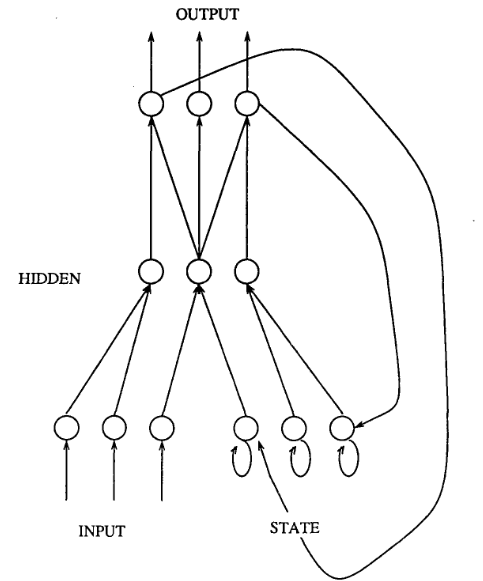
\includegraphics[width=.5\linewidth]{RNNIllustration.png}
        \caption[Schema of a Jordan Network]{Schema of a Jordan Network - \cite{elman1990finding}}
        \label{fig:RNNIllustration}
    \end{center}
\end{figure}

So, when evaluating a sample, the input layer receives not exclusively the values of the independent variables of the sample, but also some values that depend on its state at previous times.

The ability to modify the output depending on the previous sample evaluated is what allows the to have some type of memory.
Models that are able to take don't evaluate each sample independently but are instead able to take into account a context, are useful for applications such as Natural Language Processing (NLP).

This is due to the fact that when trying to predict the next word in a sentence for example, it is important to take into account evey previous word \cite{tarwani2017survey}.
A backpropagation neural network, due to its nature, would only be able to take into account a fixed number of words.

Nowadays, other methods beyond SRNNs are used to do this task.
Most notably, in the last few years, Transformers\cite{vaswani2017attention} became very popular.
Nevertheless, models that are able to take into account a sequence of samples are still very much needed.

In the context of hard drive failure prediction, our samples are not words, but they do consist on a time series and thus form a well defined sequence.
This indicates that SRNNs may be a good model to tackle the problem.

Indeed, Xu et al \cite{Xu16} made use of Recurrent Neural Networks to the problem at hand.
Their setup for the neural network is quite standard, up until the point in which they introduce the concept of health status.

So, differently from every other approach in the litterature they do not divide the samples on good or failing.
They actually use a more general method in which samples are divided in $N$ classes.

The ones from hard drives that do not fail during the observation period are given the label $N-1$.
The samples from failing disks are divided in the other $N-1$ classes, labeled from $0$ to $N-2$.
The algorithm they use to assign the failing samples divides them depending on how close they are to the failure by using fixed-length intervals.

We can formally define the approach that they explained in natural language in their paper as follows:
suppose that the last $n$ samples from each failing disk are kept and need to be divided in $N-1$ bins numbered from 1 to $N-1$.
Let the last sample from a specific hard drive before it fails be taken at time $T_i$.
Then, supposing that a sample is taken every 1 unit of time (usually once per hour) the class $c_i(t)$ of the sample of the disk $i$ at time $t$ is given by:

\begin{equation}\label{eq:linear_discrete_health_status}
  c_i(t) = 
  \begin{cases}
    & N-1 \text{, if } i \in \mathbf{good} \\
    & \biggl\lfloor(T_i-t)\dfrac{(N-1)}{n}\biggr\rfloor, 0 \leq T_i - t < n \text{, if } i \in \mathbf{bad}
  \end{cases}
\end{equation}

Here, $\lfloor x \rfloor$ is the floor of $x$, meaning the largest integer smaller than or equal to $x$.
For example, $\lfloor 1.8 \rfloor = 1$, $\lfloor 3 \rfloor = 3$.

By analizing this formula, we see that the $\dfrac{n}{N}$ samples closest to the moment of failure are assigned to class 1, the next $\dfrac{n}{N}$ are assigned to class 2 and so on.

We can also prove that the formula indeed does what is desired, that is, it assigns a number from 0 to $N-2$ to each sample.
In order to do so, we notice that since we have $n$ samples taken every 1 unit of time, and the last one is taken at time $T_i$, the first one is taken at $T_i - n + 1$.

We can compute $c_i(T_i) = 0$ and $c_i(T_i - n + 1) = \biggl\lfloor(N-1)\left(1-\dfrac{1}{n}\right)\biggr\rfloor + 1$.
Since $\left(1-\dfrac{1}{n}\right) < 1$, $\biggl\lfloor(N-1)\left(1-\dfrac{1}{n}\right)\biggr\rfloor < N - 2$.
Moreover, $c_i(t)$ is clearly monotonic, since it is a composition of the floor function and elementary mathematical operations.

So, we can guarantee that the formula given above for $c_i(t)$ correctly assigns each sample to a class from $0$ to $N-2$ in which the closer the sample is to the moment the drive fails, the smaller is the value of its class label.

Here it is important to stress that the implementation of health status on the study by Xu et al \cite{Xu16} is different from the one by Li et al. \cite{Li14} that used this concept to train their decision trees.
The main distinction is that the later used continuous values in order to train a regression tree.
The former, on the other hand, divides the samples in discrete classes.

So, when training the recurrent neural network model, the $N$ classes are completely independent.
Concretely, it does not use the fact that when the correct output for a certain sample is 1, it is better to classify it as belonging to class 2 than to class $N$.

Even though the health status is a useful abstraction, in the end there is a need to output a prediction of whether the sample belongs to the \textbf{good} or \textbf{bad} hard drive.
In other words, the model needs to state if the hard drive is going to fail soon or not which is the actual problem we are trying to solve.

In order to do that, when they want to predict the status of a certain drive, they take its last $N$ samples.
Then, in order from the oldest to the most recent they put each sample as input to the network.
The order in which they are evaluated is important, since the model being used is an RNN and therefore has memory.

For each sample, they classify it as belonging to the class whose associated output neuron value is maximum.
By doing this, it is obtained a sequence of integers $c = (c_1, \dots, c_n), 1 \leq c_i \leq N$.

For each $j \in \{1,\dots,N\}$, let $C_j$ be the cardinality of $j$ in $c$.
It is clear that $\sum_{j=1}^N C_i = n$.
Then, they define two algorithms, the Voting Algorithm which Tends to Health (VAT2H) and the Voting Algorithm which Tends to Failure (VAT2F):

% TODO: explain how this differs from the algorithm we used  (sum of probabilities instead of sum of classes)

\begin{equation}\label{eq:vat2h}
    \text{VAT2H}(C) = 
    \begin{cases}
        & \text{Healthy, if } \sum_{j=1}^{N-2}C_j \leq C_N \\
        & \text{Failure, otherwise}
    \end{cases}
\end{equation}

\begin{equation}\label{eq:vat2f}
    \text{VAT2F}(C) = 
    \begin{cases}
        & \text{Healthy, if } \sum_{j=1}^{N-2}C_j < C_N \\
        & \text{Failure, otherwise}
    \end{cases}
\end{equation}

Notice that the contribution of the class $N-1$ is ignored in both algorithms.
This implies that these algorithms only work for when $N \geq 3$.

So, in order to tackle the problem they start by expanding the number of classes from 2 to $N$ using equation \ref{eq:linear_discrete_health_status}.
Then, after the network classifies a sequence of samples of the same disk in the classes from 1 to $N$ they use equation \ref{eq:vat2h} or \ref{eq:vat2f} to obtain the final binary classification output.

They perform their tests on three different datasets corresponding to different models of hard drives.
% TODO: add a source for these claims
The neural network for each model is trained independently since, as discussed, not only the behavior of hard drives of different models can be different, but also, for different vendors, the values of the SMART attributes are not guaranteed to be compatible.

They obtained promising results of their approach.
The FDR of their models was around 97\% while the FAR was almost always kept below 0.1\%.
As was expected, the VAT2H algorithm resulted in a lower FDR and a lower FAR than the VAT2F algorithm.

Nevertheless, their study admitted to having some limitation such as not studying the impact of other health status algorithms different from the one in equation \ref{eq:linear_discrete_health_status}.
Moreover, they used a fixed amount of classes with $N=6$ all over their research as well as a constant number of nodes in the hidden layer of their network.

\section{Long Short-Term Memory Network}\label{sec:lstm}

Time has proved that RNNs are an effective method to tackle multiple sequence-based problems such as NLP \cite{tarwani2017survey} and video processing \cite{yadav2022survey}.

However, RNNs suffer from a limtation called the vanishing gradient problem.
This limits their efficiency when they need to learn long term dependencies.

This has been proven theoretically by Hochreiter \cite{hochreiter1998vanishing} as well as by Bengio using different approaches \cite{bengio1993problem}.
The intuition behind this result can be explained using the concept error signal defined in Equation \ref{eq:error_signal}.

If we expand the bottom expression to explicitly write $e_i^{(l)}$ in terms of the error signals of layer $l+2$ instead of $l+1$, we obtain:

$$
    e_i^{(l)} = \varphi '(u_i^{(l)}) \sum_j w_{ij}^{(l)} \varphi '(u_j^{l+1}) \sum_k w_{jk}^{(l+1)} e_k^{l+2}
$$

From this, we can see that $\dfrac{e_i^{(l)}}{e_i^{(l+2)}} \propto \varphi '(u_i^{(l)})\varphi '(u_j^{l+1})$.
So, it is proportional to the product of two derivatives.
We can exend this process to show that the impact induced by layer $l + m$ on layer $l$ must be scaled by the product of $m$ derivatives.

% TODO: draw a schema representing backpropagation through time (just multiple copies of the same network)
But, if we redraw our RNN to be represented by Figure , we see that the input of sample $t$ can be interpreted as being connected to the imput of sample $t'$ by $(t'-t+1)k$ layers.
So the impact of the sample $t$ on sample $t'$ is proportional to $\prod_{i=1}{(t'-t+1)k}\varphi'(x_i)$.

But, if the values of $\varphi'(x_i)$ are all smaller than 1, not only the scaling term will approach 0, but it will do so exponentially fast with respect to the distance between the two samples.

What Bengio showed on his paper \cite{bengio1993problem} is that, as a network learns, these derivatives decrease and become smaller than 1.
From this result, he was able to prove that as the distance between two samples increase, the impact of the earlier one on the other on the RNN tends to zero, as long as the network has enough time to learn.

The only assumption he made was that the model was not sensitive to noisy perturbations.
This is equivalent to stating that if two data sets are similar, then the model is able to learn approximately the same pattern, which is coherent to the problem at hand.

So, there is a theoretical demonstration that for long enough sequences, the RNN architecture will be subjected to the vanishing gradient problem.
However, theory alone is not enough to define what is a long enough sequence.
In order to state that the vanishing gradient problem has an impact on RNNs it is needed to observe such phenomenon in real-world scenarios. 

And, indeed, experiments show that problems as diverse as sentiment analysis (\cite{raza2021cloud}) and greenhouse gas predictions (\cite{ludwig2019comparison}) can be better learned by networks that try to solve the vanishing gradient problem such as LSTMs.

Other research projects show that applying techniques explicitly developed to curb the vanishing gradient problem can result in better results even without needing to change the architecture at all.
For instance, in \cite{hu2021handling} they adapted the activation functions that increase the value of their derivatives.

With this evidence, both theoretical and experimental, it is clear the need to develop networks that are able to better handle or completely avoid the vanishing gradient problem.

So, after proving the vanishing grdient problem in RNNs, Hochreiter developed a network that was not subjected to the same problem.
His solution was the Long Short-Term Memory architecture (LSTM).
A schematic view of such network is presented on Figure \ref{fig:LSTMSchema}.

\begin{figure}
    \begin{center}
        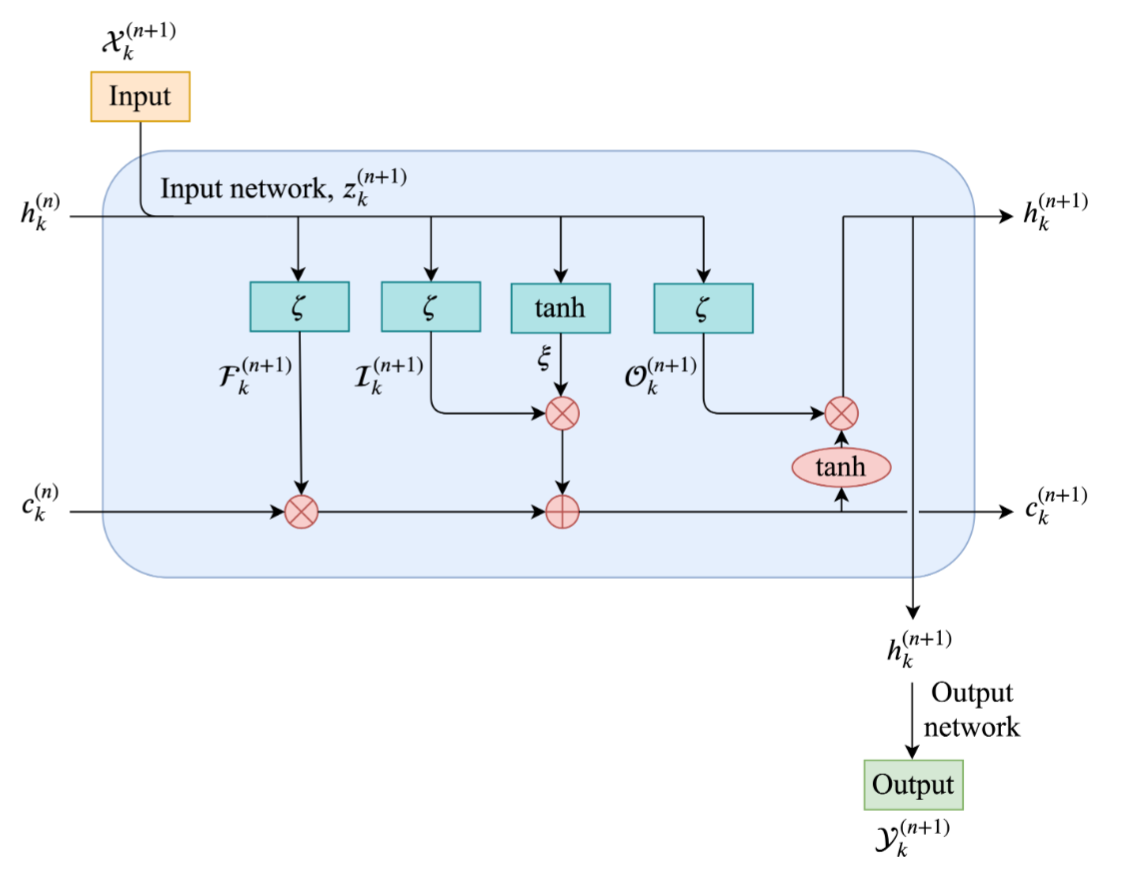
\includegraphics[width=.6\linewidth]{LSTM-Schema.png}
        \caption[Schema of an LSTM]{Schema of an LSTM - \cite{rahman2019nonintrusive}}
        \label{fig:LSTMSchema}
    \end{center}
\end{figure}

Simillarly to the RNN architecture, we combine the output of the previous sample (represented by $h^{(n)}$ on the image) with the input data for the current sample ($\chi^{(n+1)}$).
However, the main innovation is the presence of the cell state, the channel represented by the horizontal lane in the bottom half of the image and dented by $c^{(n)}$.

It is not updated using the same logic of the neurons used by BPNNs and RNNs so it is not subject to the vanishing gradient problem.
The operations performed by an LSTM can be explained in three steps, each one called a gate.

The first one is called the forget gate and is represented in the image by the leftmost $\zeta$ node.
It takes the input of the current sample ($\chi^{(n+1)}$) and the last output ($h^{(n)}$) of the network and generates a forget factor vector $P^{(n+1)}$ which is then multiplied component by component with the current value of the state $c^{(n)}$.

The name from this gate comes from the fact that it controls how much the network remembers from the past samples.
In the limit case in which $P^{(n+1)} = \mathbf{0}$, the value of $c$ is reset and no information is kept from previous interations.

The next step is the input gate, which in the image corresponds to the central $\zeta$ and $\tanh$ nodes.
If the forget gate decides how much from previous iterations should be kept in the cell state, the input gate controls which data from the current one should be added to the cell state.

The input gate is divided in two steps: the first is to generate the candidate values $\xi$ and the second is to compute the weights $I^{(n+1)}$.
Then each component of the candidate values vector is multiplied by its corresponding weight and added to the cell state.

Finally, there is the output gate that will actually compute the predicted ouput value for the sample.
In the image it is represented by the rightmost $\zeta$ and $\tanh$ gates.

This is the step that uses the cell state as input.
It combines the cell state value as well as the sample input $x^{(n+1)}$ and the previous sample output $h^{(n)}$ to compute a prediction $h^{(n+1)}$ for the current sample. 

In the previous paragraphs, we used generic terms such as compute and generate.
However, for an LSTM, the equations to calculate each term presented above is well defined and are given by:

\begin{equation}\label{eq:lstm_calculations}
    \begin{cases}
        P^{(n+1)} &= \zeta(W_f\cdot[h^{(n)}, x^{(n+1)}] + b_f) \\
        I^{(n+1)} &= \zeta(W_i\cdot[h^{(n)}, x^{(n+1)}] + b_i) \\
        \xi &= \tanh(W_\xi\cdot[h^{(n)}, x^{(n+1)}] + b_\xi) \\
        C^{(n+1)} &= P^{(n+1)} \odot C^{(n)} + \xi \odot I^{(n+1)} \\
        O^{(n+1)} &= \zeta(W_o\cdot[h^{(n)}, x^{(n+1)}] + b_o) \\
        h^{(n+1)} &= O^{(n+1)} \odot \tanh(C^{n+1})
    \end{cases}
\end{equation}

In the equation above, $[x, y]$ is the concatenation of vectors $x$ and $y$ and $x \odot y$ is the Hadamard or element-wise product.
Also, $W_x$ and $b_x$ represent, respectively, the weights and bias of the network when computing variable $x$.
These are the values that need to be learned during the training process.

When it comes to applying this architecture to solving the problem of prediciting hard drive failure in data centers, there are not many research projects that focused in this problem that have been published.
Nevertheless, there are some related works.

The first of them was done by Zhang et al. (\cite{zhang2017deep}).
The main objective of their work was to develop a symbolization-based feature extraction algorithm to improve event detection in LSTMs.

To show the impact of their approach they did perform an experiment on hardware failure detection.
However, they were presenting a more general method.
Consequently, they used different metrics such as balanced accuracy instead of FAR and FDR that would allow us to directly compare with other methods.

Despite us not having access do the desired metrics we can deduce some aspects of their results that allow us to compare to other works.
In order to do that, let positive be the event of the hard drive failing and negative the event of it not failing.

Then the true positives $TP$ are the hard drives whose failure was correctly predicted.
The true negative $TN$ are the hard drives that did not fail and that were not flagged as going to fail.
The false negatives $FN$ are the hard drives that failed but were not flagged as so.
And, the false positives $FP$ are the hard drives that did not fail but that were predicted as going to fail.

This allows us to rewrite the FDR and the FAR as follows:

\begin{equation}
    \begin{cases}
        \begin{aligned}
            FDR &= \dfrac{TP}{TP + FN} \\
            FAR &= \dfrac{FP}{FP + TN}
        \end{aligned}
    \end{cases}
\end{equation}

We then introduce the definition of Balanced Accuracy(BA), which was the metric used in \cite{zhang2017deep}:

\begin{equation}\label{eq:ba_def}
    BA \equiv \dfrac{1}{2}\left(\dfrac{TP}{TP + FN} + \dfrac{TN}{TN + FP}\right)
\end{equation}

But by manipulating \ref{eq:ba_def}, it is possible to rewrite it in terms of the FDR and the FAR:

\begin{equation}
    BA = \dfrac{FDR + (1-FAR)}{2}
\end{equation}

So, even though it is not possible to retrieve the FDR and the FAR by themselves, it is possible to find a range of possible values for them from the balanced accuracy value.

In \cite{zhang2017deep}, the best BA they achieved over all the experiments with the LSTMs, with or without their feature extraction algorithm, was $85.2\%$.
But, since BA is the average of FDR and $(1-FAR)$, it implies that one of these values is at most $85.2\%$, else their average would be bigger.

So, either the FDR they achieved is under $85.2\%$ or their FAR is above $14.8\%$ which is much worse than the one achieved with any other methods we have discussed.

This indicates that their research cannot be used as a reference for the hard disk failure detection problem.

There is an additional paper by Das et al. (\cite{das2018desh}) that also applies LSTM to hardware failure detection.
However, it is not for hard drives in data centers, but rather to nodes in a supercomputer which leads to a profile much different than the papers discussed so far.

The first main difference is that the time scales in which it operates is much smaller.
The TIA they achieve is of the order of 100 seconds, which indicates a very different behavior than the one found in data centers in which it is possible to predict a failure more than 100 hours in advance (\cite{Li14}, \cite{Zhu13}).

But the most important difference is that in \cite{das2018desh} they try to predict failures that happen in components other than the hard drive.
So, they do not make use of SMART attributes, they instead analyze system logs.

Therefore, their motivation to use LSTMs is to detect patterns in text rather than to study time-series.

The FDR they achieve with their LSTM-based approach is between $85.1\%$ and $87.5\%$.
However it is not possible to compare it to the other results presented above since their problem is quite different from the detection of hard drive failures in data centers.

\section{Other Techniques}

There are three additional methods that have been used to tackle the hard drive failure prediction problem and that are worth mentioning.
Since these approaches will not be implemented by our current work, we will limit ourselves to a briefer explanation of the theory behind them.

\section{Random Forest}\label{sec:randomforest}

One of the problems faced by Decision Trees, specially when they become large is overfitting \cite{ying2019overview}.
This is due to the fact that the split values for each attribute used by the tree are directy taken from the values on the training set.
So, when the tree is deep and there are only a few training samples in a node, the splitting values will sharply follow the ones in the training set.

Another way to explain this is that since a Decision Tree can closely follow the patterns observed in the training set because it can choose the splitting threshold independently of the ancestor nodes in the tree, it presents a small bias.
But in Machine Learning there is a principle known as the Bias-Variance tradeoff that states that a model with low bias will present a high variance and vice-versa \cite{briscoe2011conceptual}.

More concretely, for our problem at hand, suppose that there are only a few samples in the training set with a certain cause of failure.
During training, if they are in a node $\mathbf{N}$ and are mixed with other samples, we may be able to correctly put them in a leaf that is a child of $\mathbf{N}$.

So, the model will have a good performance on the training set which corresponds to a small bias, since the expected and predicted value will be the same.
However, imagine that when evaluating an unseen sample there is an attribute, that is not important, to identify this cause of failure, is slightly different from the values observed in the training set.

Then, the path taken will not go through $\mathbf{N}$ and thus it won't go through the same evaluation process as samples that are simillar.
As a result, a small change in a random attribute can cause a huge differnce on the path traversed and thus on the result.
Having an algorithm that can behave very differently for slightly different inputs corresponds to a model that has a high variance.

In order to tackle this, the concept of Random Forests has been introduced \cite{ho1995random}.
The idea is to train multiple, independent Decision Trees at once, each one trained with a different subset of the training data.
Notice that these subsets do not have to be disjoint, specially when the train set is relatively small.

Random Forests have performed well for a variety of tasks, ranging from image recognition to Alzheimer's disease detection and prediction \cite{shaik2019brief}.

The set of trees has, therefore, a smaller bias when compared to the one trained using all the data at once.
This is due to the fact that we can reduce the probability of overfitting, since there will have a larger varierty of decision nodes.

If we return to the example of a specific cause of failure, the training samples corresponding to it will not even necessarily be on the same tree anymore.
So, there is a larger set of nodes that have been trained with samples corresponding to this failure.
Therefore, the probability of going through one of them when traversing the tree is higher even if the unseen sample does not correspond perfectly.

The drawback is that since the training samples with the same failure cause will be spread, the probability of having a node that had multiple ones when training is smaller, which can increase the error on the training set and on samples very simillar to the ones in the training set.

Once the set of trees is created and trained, it remains to decide how to regroup all of them.

The most common approach when asking for the model to predict the result for a sample is to take the value predicted by each tree and then combine them.
For a classification problem, it can be returning the most common predicted class, while for a regression problem it can be done by taking the average of the outputs of the trees.

This can be done quite efficiently, since, at each node, it suffices to compare the value of a specific attribute with a threshold and go to the corresponding child.
Moreover, since the traversal processes are independent, they can even be done in parallel.

A research by Shen et al. \cite{Shen18} used Random Forests for hard drive failure prediction.
One of the most interesting aspects of their research is how they combined the results of the different tree of the forests.

Instead of simply checking whether most trees had an output of \textbf{good} or \textbf{bad} for a specific sample, they giving different trees different weights based on a clustering algorithm.

More specifically, they performed the clustering process for the good and bad samples independently.
Then, when predicting the outcome for an unseen sample, the clusters $c_1$ and $c_2$ to which it would belong if it were a good or bad one are computed.

Since it is known which samples of the training set were used to train each tree, it is possible to evaluate the accuracy of each tree for the training samples in $c_1$ and in $c_2$.
Based on these accuracies, it is possible to give a bigger weight to trees that better learned the samples of the clusters to which the sample being evaluate belongs.

They used a simple algorithm in which the weight of a tree is either $0$ or $1$ depending on whether its accuracy for its training sample belonging to either $c_1$ or $c_2$ is at least $0.5$.
However, it is not difficult to imagine a slightly more complex algorithm that results in a weight $w \in \left[0,1\right]$ which is directly proportional to the accuracy.

Despite this simplicity, they were able to achieve a great performance.
The FDR obtained was above 98\% while the FDR was kept under 0.1\% for multiple scenarios.

What allowed them to get these excellent outcomes, besides of course the algorithm, was their dataset that contained more than 2 million samples of SMART attribute snapshots.

\subsection{Support-Vector Machine}

A Support-Vector Machine (SVM) is a non-probabilistic classifier \cite{cortes1995support}.
The idea behind it is to plot the samples in an n-dimensional space, in which $n$ corresponds to the number of features in the vector.

Then, the algorithm finds the hyperplane that minimizes its loss function.
The points on one side of the hyperplane correspond to the positive class and the other to the negative class.

The main drawback of SVMs is that drawing a hyperplane means that it can only detect linear dependencies.
So, if there are points in a 2D-plane and the boundaries between the good and bad class is the circumference centered at the origin with radius 1, there is no way that a line can be drawn to correctly divide both regions.

The solution to this is to use the kernel-method, in which dimensions of the original vector are combined using non-linear function and the output of the function is assigned to a new component of the sample vector.
This allows the SVM to correctly learn non-linear dependencies between the variables.

In the example above, we can transform the vector $v = (x, y)$ into $v' = (x, y, x^2 + y^2)$ and then and apply the SVM to the set of $v'$.
Then the SVM can correctly generate the plane $x_3 = 1$ and thus solve the classification problem without needing to learn explicitly non-linear dependencies.

When it comes to applying SVMs to predicting hard drive failure, the best results were achieved in \cite{Zhu13}.
They used hyperparameters on their model in order to prioritize either a small FAR or a big FDR.

When optimizing for the smallest FAR possible, Zhu et al. obtained a FAR of $0.03\%$ and an FDR of $68.5\%$.
When priority was giving to increasing the FDR, they obtained a FAR of $0.3\%$ but the FDR was increased to $80.0\%$.

Support-Vector Machines, when compared to other approaches, present, therefore, a method that is able to achieve a smaller FAR.
However, in contrast, it is not able to attain FDRs as good as other methods while keeping an acceptable FAR.

In the research by Zhu et al. they kept results that had an FAR smaller than $5\%$, so it implies that improving the FDR above $80\%$ requires increasing the FAR to unacceptable levels.

\subsection{Convolutional Neural Networks}

A Convolutional Neural Network (CNN) is a deep learning machine learning model.
It is usually applied to computer vision tasks.
Just like BPNNs discussed in Section \ref{sec:BackpropagationNeuralNetwork}, it is not recurrent meaning that the output for a certain sample is not propagated to following ones.

The main aspect that differs a CNN from a BPNN is the presence of convolutional layers \cite{o2015introduction}.
In a convolutional layer, a neuron in layer $l$ is not connected to every neuron in layer $l-1$.
Instead, it is connected to a few consecutive nodes of layer $l-1$.

This is useful for handling data with many input parameters, such as images, in which each pixel corresponds to an input.
For a 100x100 image, fully connecting two layers would require 10,000 weights.
By using a 5x5 convolution window with shared weights, it is possible to reduce this value to only 25 weights, or 400 times less.
This allows the network to be much deeper.
 
A relevant attribute of a CNN is its translation invariance \cite{kayhan2020translation}.
The use of shared weights implies that shifting some values by a certain constant value does not hinder the network's ability to recognize a certain pattern.
This is because the convolutions will be performed with the same weights no matter in which part of the image a certain sequence of values is.

It was exactly this aspect of the CNN that motivated Sun et al. (\cite{sun2019system}) to adapt CNNs to handle time series in order to tackle the hard drive failure prediction problem.
For a time-series, translation invariance implies that a pattern due to a sequence of values or events can be detected indepndently of where in the sequence it occurs.

In order to obtain, they also had to adapt the loss function to handle the imbalanced dataset that contained many more good samples than failing ones, which is an intrisic aspect of the problem at hand.

So, they gave a bigger weight to failing samples that were misclassified, else the model would be prone to classify almost every disk as a good one.
This is due to the fact that, with a classic loss function, even if the model misclassified every failing disk, its total loss would be much smaller than if it misclassified even a small percentage of the good disks.

In their results, the metric they presented that we can use to compare with other methods was the precision, which corresponds to the FDR.
They achieved a FDR of $75\%$ which is considerably smaller than the one attained by other models.

But this is mainly due to the fact that they used an heterogeneous dataset, meaning that they did not train different networks for different hard drive models.
So, it is difficult to compare this results with the ones presented so far.